% !TEX root = main.tex
Today's complex cyber-physical systems are characterized by the interaction of a large number of heterogeneous components. Consequently, the models used to analyze these systems are equally complex and consist of heterogeneous sub-models relying on different assumptions and based on principles from different scientific disciplines. It is not uncommon to encounter a patchwork of differential equations, difference equations, hybrid automata, lookup tables, custom switching logic, low-level legacy code, etc. To further compound the difficulty in analyzing these systems, different components of a complex engineered system are typically designed by different suppliers. Although a high-level specification for these components may be known, detailed models are not available for intellectual property reasons. We are thus faced with a tremendous gap between the existing analysis techniques that rely on closed-form models and the models available in industry. It is, therefore, not surprising the emphasis that industry places on simulation since despite the complexity of models, it is always possible to simulate them. This raises the question of whether we can provide formal guarantees about certain properties of these complex systems based solely on the information obtained via their simulations. In this paper, we focus on one of the most important of such properties in the context of control theory: stability.


More formally, we consider a dynamical system as in:
\vspace{-0.88394mm}
\begin{equation}\label{eq:dynamicalsystemGeneral}
x_{k+1} = f(k, x_k),
\end{equation}
where, $x_k \in X$ is the state and $k \in \mathbb{N}$ is the time index. 
\textcolor{red}{Rajout: If \eqref{eq:dynamicalsystemGeneral} is linear, its identification and stability analysis have been extensively studied. In this work, we take a first step into more complex systems by considering the class of switched linear systems. Although we restrict ourselves to such systems, we believe that the presented results can be extended to more general classes of dynamical systems.} 
%We restrict ourselves to switched systems in this work, but we believe that the presented results can be extended to more general classes of dynamical systems.
We start with the following question to serve as a stepping stone: For some $l \in \mathbb{N}_{>0}$, given $N$ traces of length $l$, $(x_0^i,x_1^i,\dots, x_l^i)$, ($1 \leq i leq N$), belonging to the behavior of the system \eqref{eq:dynamicalsystemGeneral}, (i.e., $x_{k+1}^i = f(k, x_k^i)$ for any $k \in \{0,\dots,l-1\}$ and any $i \in \{1,\dots,N\}$), what can we say about the stability of the system \eqref{eq:dynamicalsystemGeneral}? For the rest of the paper, we use the term \emph{black-box} to refer to systems where we do not have access to the model, i.e., to $f$, yet we can indirectly learn information about $f$ by observing traces of length $l$ (in the particular case of $l=1$, these traces become couples of points $(x_k, y_k)$ as defined in \eqref{eq:dynamicalsystemGeneral}).
%\textcolor{red}{We should say that this is non-ideal when we don't know what the state is, but it is a start, and it makes sense in certain situations. Paulo's comment: If we don't have a model, then we don't know what the state is. But the issue I raised is even deeper. Why can we assume that we can initialize the state randomly? Joris' comment: we do not necessarily assume that WE initialize the set randomly. We have random observations of the state, we do not know the process that picks the state, and we model this process with a random distribution. By default we take it uniform since we cannot say some states are privileged a priori. But a future step would be to consider different distributions and extend our guarantees to them.}

A potential approach to this problem is to first identify the dynamics, i.e., the function $f$, and then apply existing techniques from the model-based stability analysis literature. However, unless $f$ is a linear function, there are two main reasons behind our quest to directly work on system behaviors and bypass the identification phase: 
\begin{itemize}
\item Even when the function $f$ is known, in general, stability analysis is a very difficult problem \cite{stabilityHard1}; 
\item Identification can potentially introduce approximation errors, and can be algorithmically hard as well. Again, this is the case for switched systems \cite{lauer}. 
\end{itemize}

A fortiori, the combination of these two steps in an efficient and robust way seems far from obvious.

In recent years, increasing number of researchers started addressing various verification and design problems in control of black-box systems \cite{bianchini, balkan, mitra, mitra2}, \textcolor{red}{Do we add the HSCC '16 paper \cite{kozarev2016case} on machine learning for abstractions here?}. In particular, the initial idea behind this paper was influenced by the recent efforts in \cite{topcu, kapinski}, and \cite{lazar} on using simulation traces to find Lyapunov functions for systems with known dynamics. In these works, the main idea is that if one can construct a Lyapunov function candidate decreasing along several finite trajectories starting from different initial conditions, it should also decrease along every other trajectory. Then, once a Lyapunov function candidate is constructed, this intuition is put to test by verifying the candidate function either via off-the-shelf tools as in \cite{topcu} and \cite{kapinski}, or via sampling-based techniques as in \cite{lazar}. This also relates to almost-Lyapunov functions introduced in \cite{liberzon}, which presents a relaxed notion of stability proved via Lyapunov functions decreasing everywhere except on a small set. Note that, since we do not have access to the dynamics, these approaches cannot be directly applied to black-box systems. However, these ideas raise the following problem that we address in this paper: By observing that a candidate Lyapunov function decreases on a large number of observations, we empirically build a certain confidence that such candidate Lyapunov function is a bona-fide Lyapunov function. \emph{Can we translate this confidence into a confidence that this Lyapunov function decreases at most of the points in the state space?} 

Note that, even in the case of a 2D linear system, the connection between these two beliefs is nontrivial. In fact, one can easily construct an example where a candidate Lyapunov function decreases everywhere on its levels sets, except for an arbitrarily small subset, yet, almost all trajectories diverge to infinity. For example, the system
\[
x^+ = \begin{bmatrix}
0.14 & 0\\
0 & 1.35
\end{bmatrix}x,
\]
admits a Lyapunov function candidate on the unit circle except on the two red areas shown in Fig. \ref{fig:levelset}.
Moreover, the size of this ``violating set" can be made arbitrarily small by changing the magnitude of the unstable eigenvalue. Nevertheless, the only trajectories that do not diverge to infinity are those starting on the stable eigenspace that has zero measure.
\begin{figure}[H]
\centering
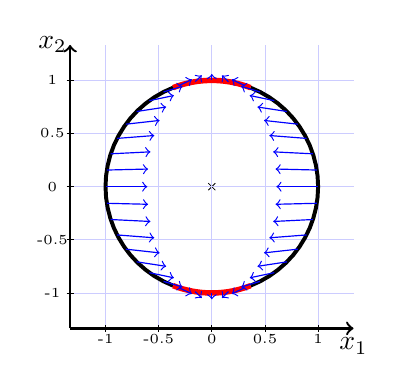
\begin{tikzpicture}[scale=0.45]
\draw[line width = 0.3mm,black,->] (-4,-4) -- (4,-4);
\draw[line width = 0.3mm,black,->] (-4,-4) -- (-4,4);

\draw (4,-4.5) node {$x_1$};
\draw (-4.5,4) node {$x_2$};
\draw[line width=0.1mm,black] (-0.1,-0.1) -- (0.1,0.1);
\draw[line width=0.1mm,black] (-0.1,0.1) -- (0.1,-0.1);

\foreach \i in {-2,...,2}
{
\draw[line width=0.1mm,blue!20] ({1.5*\i},-3.9) -- ({1.5*\i},4);
}

\foreach \i in {-2,...,2}
{
\draw[line width=0.1mm,blue!20] (-3.9,{1.5*\i}) -- (4,{1.5*\i});
}

\draw [line width = 0.5mm,black,domain=-68.66:68.66] plot ({3 * cos(\x)}, {3 * sin(\x)});
\draw [line width = 0.7mm,red,domain=68.66:111.34] plot ({3 * cos(\x)}, {3 * sin(\x)});
\draw [line width = 0.5mm,black,domain=111.34:248.66] plot ({3 * cos(\x)}, {3 * sin(\x)});
\draw [line width = 0.7mm,red,domain=248.66:291.34] plot ({3 * cos(\x)}, {3 * sin(\x)});

\foreach \i in {-2,...,2}
{
\draw[line width=0.1mm,black] ({1.5*\i},-4.1) -- ({1.5*\i},-3.9);
}

\draw (0,-4.3) node {\tiny{0}};
\draw (-1.5,-4.3) node {\tiny{-0.5}};
\draw (-3,-4.3) node {\tiny{-1}};
\draw (1.5,-4.3) node {\tiny{0.5}};
\draw (3,-4.3) node {\tiny{1}};

\foreach \i in {-2,...,2}
{
\draw[line width=0.1mm,black] (-4.1,{1.5*\i}) -- (-3.9,{1.5*\i});
}

\draw (-4.5,0) node {\tiny{0}};
\draw (-4.5,1.5) node {\tiny{0.5}};
\draw (-4.5,3) node {\tiny{1}};
\draw (-4.5,-1.5) node {\tiny{-0.5}};
\draw (-4.5,-3) node {\tiny{-1}};

\foreach \i in {0,...,39}
{
\draw[line width =0.15mm,->,blue] ({3*cos(\i*9)},{3*sin(\i*9)}) --  ({3*cos(\i*9)-2*0.19661*3*cos(\i*9)},{3*sin(\i*9)+2*0.03001*3*sin(\i*9)});       
}
\end{tikzpicture}
\caption{A simple dynamics and the level set of an ``almost Lyapunov function''. Even though this function decreases at almost all points in its level set, almost all trajectories diverge to infinity.}
\label{fig:levelset}
\end{figure}
In this paper, we take the first steps to infer stability from observations of switched linear systems. In addition to the preceding example, there are other reasons to temper our expectations for proving stability from data. First,  identifying an arbitrary switched linear system is NP-hard \cite{jungers_lncis}. Second, the stability of switched linear systems is closely related to a quantity on the matrices modeling the dynamics in each mode, whose computation is itself known to be NP hard: the \emph{joint spectral radius} (JSR). Indeed, deciding stability amounts to deciding whether the JSR is less than $1$ \cite{jungers_lncis}. In this paper, we present an algorithm to bound the JSR of a switched linear system from a finite number $N$ of observations. This algorithm partly relies on tools from the random convex optimization literature (also known as chance-constrained optimization, see \cite{campi,nemirovski,campi-garatti}), and provides an upper bound on the JSR with a user-defined confidence level. As $N$ increases, this bound gets tighter. Moreover, with a closed form expression, we characterize what is the exact trade-off between the tightness of this bound and the number of samples. In order to understand the quality of our upper bound, the algorithm also provides a deterministic lower bound. Finally, we provide an asymptotic guarantee on the gap between the upper and the lower bound, for large $N$.

%\textcolor{blue}{We note that, aside from the stability analysis, black-box setting has been adopted by several researchers in the analysis and control of dynamical systems in the recent years. For example, in \cite{bianchini}, the authors consider the tuning a black-box plant by choosing suitable inputs. In \cite{balkan}, by exciting a black-box system with different inputs, authors generate test cases to challenge the system with respect to a given design specification.} \textcolor{red}{Anything more here?}

The organization of the paper is as follows: In Section~\ref{sec:preliminaries}, we introduce the problem studied and provide the necessary background in stability of switched linear systems. Then, based on finite observations for a given switched linear system, we give in Section~\ref{sec:lowerBound} a deterministic lower bound for the JSR, before presenting in Section~\ref{sec:upperbound} the main contribution of this paper, which consists in a probabilistic stability guarantee. We illustrate the performance of the presented techniques with some experiments in Section~\ref{sec:experiments}, then we conclude in Section~\ref{sec:conclusions}, while hinting at our related future work.